\documentclass[10pt,a4paper]{article}

\usepackage[T1]{fontenc}
\usepackage[utf8]{inputenc}
\usepackage{polski}
\usepackage[left=1in,right=1in,top=1in,bottom=1in]{geometry}
\usepackage{lmodern}

\usepackage{graphicx}

\usepackage{booktabs}

\usepackage{enumitem}
\usepackage{import}
\usepackage{array}


\usepackage[hyphens]{url}
\usepackage[hidelinks]{hyperref}


\hypersetup{breaklinks=true}

\graphicspath{ {./img/} }

\bibliographystyle{elsarticle-num}

\renewcommand{\figurename}{Rys.}
\renewcommand{\tablename}{Tab.}


\usepackage{pythonhighlight}

\begin{document}
\begin{titlepage}
	\centering
	
\includegraphics[width=10cm]{PB_logo}\par\vspace{1cm}

	{\LARGE\bfseries Sztuczna inteligencja \par}
	\vspace{0.5cm}
	
	{\LARGE\bfseries Sprawozdanie z projektu końcowego\par}
	\vspace{1.5cm}
	
	{\Large Temat: Prezentacja możliwości biblioteki scikit-learn w projektach informatycznych, wymagających użycia drzew decyzyjnych.\par}
	\vspace{3cm}
	
	\raggedright
	
	
 	{\large Wykonujący projekt: \textbf{Adam Bajguz}\\
 			\makebox[0pt][l]{}\phantom{Wykonujący projekt: }\textbf{Magdalena Kalisz}\par}
 	\vspace{1cm}
 	
 	{\large Studia dzienne \par
	Kierunek: Informatyka \par
	Semestr: IV \hspace{2.5cm} Grupa zajęciowa: \textbf{PS1} \par
	Prowadzący ćwiczenie: \textbf{mgr inż. Dariusz Jankowski} \par}
 	
	\vfill
		
	\begin{tabular}{c}
	\today\\
	Data wykonania projektu
	\end{tabular}
	
	\begin{flushright}
	\begin{tabular}{c}
	..............................................\\
	Data i podpis prowadzącego
	\end{tabular}
	\end{flushright}

\end{titlepage}

\tableofcontents
\newpage

\section{Wstęp}
Drzewa decyzyjne to nieparametryczna nadzorowana metoda uczenia, która może być stosowana zarówno do klasyfikacji, jak i regresji. Pierwszy artykuł, który przedstawia podejście do klasyfikacji znane z drzew decyzyjn, pochodzi z 1959 roku \cite{Belson1959}. Z kolei pierwszy algorytm drzew regresyjnych został obublikowany w roku 1963 \cite{Morgan1963}.\par
\vskip 0.2in
Drzewa decyzyjne są jednym z najczęściej wykorzystywanych narzędzi do klasyfikacji danych i prognozowania z uwagi na fakt, że wiedza odkryta przez drzewo decyzyjne jest zilustrowana w hierarchicznej strukturze. Technika drzew decyzyjnych, czy też klasyfikacyjnych, pozwala m.in. na \cite{MazumdarWWW, Quinlan1986}:
\begin{itemize}
	\item wyznaczenie zasad decyzyjnych opisujących reguły przypisywania obiektów do wyróżnionych klas (zasady odwołują się do wartości atrybutów opisujących obiekty),
	\item analizę zbioru obiektów opisywanych przez przyjęty zestaw atrybutów, której celem jest doskonalenie podziału obiektów na jednorodne klasy.
\end{itemize}

\subsection{Drzewa decyzyjne w teorii decyzji i uczeniu maszynowym}
Drzewa decyzyjne to również graficzny sposób wspierania procesu decyzyjnego. Drzewo stosowane jest w teorii decyzji i ma szereg zastosowań. Może zarówno rozwiązać problem decyzyjny, jak i stworzyć plan. Metoda drzew decyzyjnych sprawdza się również w momencie rozwiązywania problemów decyzyjnych z wieloma rozgałęziającymi się wariantami oraz podejmowania decyzji w warunkach ryzyka. Drzewa znalazły zastosowanie w takich dziedzinach jak botanika i medycyna, a nawet ekonomia, gdyż są w stanie ułatwiać i usprawniać komputerowe wspomaganie procesu podejmowania decyzji \cite{Morgan1963, Quinlan1990}.

\subsection{Rodzaje drzew decyzyjnych}
Rodzaj drzewa decyzyjnego zależy od typu zmiennej docelowej:
\begin{itemize}
	\item drzewo decyzyjne zmiennych jakościowych (drzewo decyzyjne o zmiennej kategorialnej) - drzewo decyzyjne, które ma kategoryczną zmienną docelową,
	\item drzewo decyzyjne zmiennych ilościowych (ciągłych) - drzewo decyzyjne ma ciągłą (ilościową / numeryczną) zmienną docelową.
\end{itemize}\par
\vskip 0.2in

Zaletą drzew decyzyjnych jest to, że mogą modelować dowolny typ funkcji do klasyfikacji lub regresji. Do rozwiązywania problemów zarówno regresyjnych, jaki i klasyfikacyjnych służy metoda CART (rodział \ref{sub:CART}). Wyróżnia się dwa typy drzew decyzyjnych \cite{Breiman1984}:

% \begin{itemize}[label=$\cdot$]
\begin{itemize}
	\item drzewa klasyfikacyjne - służą porządkowaniu klas, charakteryzuje je kategoryczna zmienna zależna, której wartość (czyli przynależność przypadku do klasy, grupy) chcemy poznać na podstawie znajomości wartości jednej lub większej liczby predykcyjnych zmiennych ciągłych oraz, ewentualnie zmiennych kategorialnych;
	\item drzewa regresyjne - służą do przewidywania wartości zmiennej ciągłej, na podstawie znajomości wartości jednej lub większej liczby predykcyjnych zmiennych ciągłych.
\end{itemize}

\section{Budowa drzew decyzyjnych}
Drzewo decyzyjne buduje modele klasyfikacji lub regresji w postaci struktury drzewa, rozkłada zbiór danych na coraz mniejsze podzbiory. Oznacza to, że drzewem decyzyjnym jest graf-drzewo, które składa się z korzenia, węzłów, krawędzi oraz liści. Liście to węzły, z których nie wychodzą już żadne krawędzie. Korzeń drzewa tworzony jest przez wybrany atrybut natomiast poszczególne gałęzie reprezentują wartości tego atrybutu (Rys.~\ref{fig:structure}). \par
\vskip 0.2in
Drzewa decyzyjne charakteryzują się strukturą hierarchiczną (Rys.~\ref{fig:structure}). Oznacza to, że w kolejnych krokach zbiór obiektów jest dzielony, poprzez odpowiedzi na pytania o wartości wybranych cech lub ich kombinacji liniowych. W algorytmach konstrukcji drzew jednym z kluczowych elementów jest wybór kolejności cech, według których, na poszczególnych etapach, będzie dokonywany podział zbioru obiektów. Technika drzew decyzyjnych to uzupełnienie metod klasycznych. Przykładem może tu być analiza dyskryminacyjna. Hierarchiczność podejmowania decyzji jest cechą, która wyróżnia drzewo decyzyjne od innych metod \cite{Gatnar1998, AnalyticsWWW}.

\begin{figure}[ht]
	\centering
	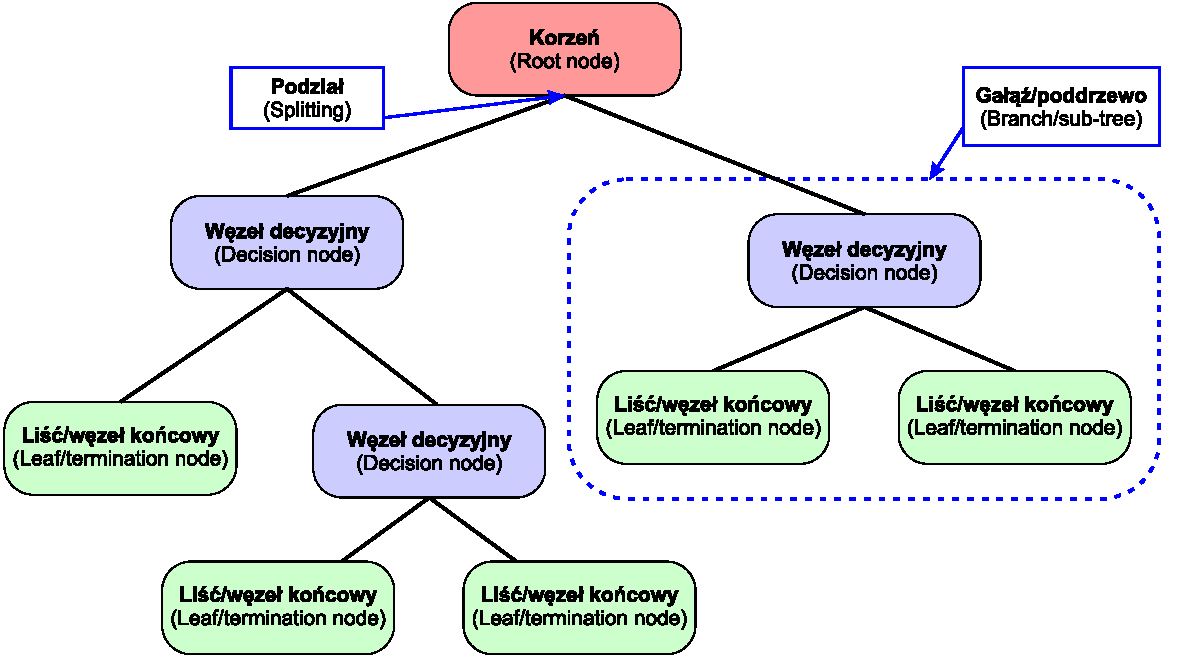
\includegraphics[width=0.9\textwidth]{structure}
	\caption{Budowa (struktura) drzewa decyzyjnego}
	\label{fig:structure}
\end{figure}


\section{Idea drzew decyzji}
Idea drzew opiera się na rekursywnym podziale danych na coraz to mniejsze sterty w celu jak najlepszego dopasowania. Drzewa decyzyjne kodują zestaw reguł if-else, które mogą być używane do przewidywania zmiennej docelowej danych funkcji danych. Reguły if-else są tworzone przy użyciu zestawu danych treningowych w celu zaspokojenia jak największej liczby instancji danych treningowych. Początkowo próbka (węzeł macierzysty, korzeń) dzielona jest na dwa lub więcej podzbiorów (węzły potomne). Natomiast węzeł optymalny wyszukuje się na podstawie wszystkich punktów węzłowych dla każdej zmiennej. Następnie proces jest powtarzany dla każdego węzła potomnego, a te podczas dzielenia traktowane są jak węzły macierzyste. Węzeł, którego nie można już podzielić nazywamy liściem, bądź węzłem końcowym, a liczbę liści - wielkością drzewa \cite{MazumdarWWW, Quinlan1986, Breiman1984, Gatnar1998, Lula2007}.

\section{Cechy drzew decyzyjnych}
Drzewa decyzyjne i uczenie się drzewa decyzyjnego razem stanowią prosty i szybki sposób uczenia się funkcji, która mapuje dane x na wyniki y, gdzie x może być mieszanką zmiennych jakościowych i liczbowych, a y może być kategoryczne dla klasyfikacji lub numeryczne dla regresji \cite{Breiman1984}.\par
\vskip 0.2in
Największą zaletą drzew decyzyjnych jest to, że mogą modelować dowolny typ funkcji do klasyfikacji lub regresji, czego inne techniki nie potrafią. Ponadto drzewa decyzyjne są uważane za metodę nieparametryczną, co oznacza nie mają one żadnych założeń co do rozkładu danych i struktury klasyfikatora. Drzewa decyzyjne zapewniają również znacznie szybsze trenowanie w porównaniu z prostymi sieciami neuronowymi przy porównywalnej wydajności (złożoność czasowa drzew decyzyjnych jest funkcją zależną od liczby cech oraz wierszy w zestawie danych, podczas gdy dla sieci neuronowych jest funkcją zależną od liczby cech, wierszy w zestawie danych, warstw ukrytych oraz węzłów w każdej ukrytej warstwie). Wadą drzew decyzyjnych jest podatność na przeuczenie. Zatem drzewa decyzyjne są używane najczęściej w przypadku bardzo dużych zbiorów danych, które są uważane za dobrze reprezentujące rzeczywistość. Niektóre algorytmy przycinania drzew są używane do rozwiązania problemu przeuczenia \cite{MazumdarWWW, Breiman1984, AnalyticsWWW, Lan2017}.

\section{Rodzaje kryteriów podziału}
W procecie budowy drzewa decyzyjengo należy wielokrotnie dokonać podziału zbioru danych, tj. należy zadać więcej niż jedno pytanie: co jest cechą, od której powinniśmy zacząć (węzeł główny) i w jakiej kolejności powinniśmy budować węzły wewnętrzne, to znaczy używać opisowych cech, aby podzielić zbiór danych? W związku z tym przydatne byłoby zmierzenie "informatywności" funkcji i wykorzystanie tej funkcji z największą "informacyjnością" jako cechą, która powinna być używana do dzielenia danych. 

\subsection{Współczynnik Giniego}
Współczynnik Giniego lub indeks Giniego to miara koncentracji (nierównomierności) rozkładu zmiennej losowej. Nazwa współczynnika pochodzi od nazwiska jego twórcy, włoskiego statystyka Corrado Giniego. Jest on wykorzystywany przez algorytm CART do mierzenia tego, jak często losowo wybrany element z zestawu byłby niewłaściwie oznaczany, gdyby był losowo oznaczony zgodnie z rozkładem etykiet w podzbiorze. Gini index można obliczyć, sumując prawdopodobieństwo $p_{i}$ elementu o etykiecie $i$ wybieranej razy prawdopodobieństwo 
$\sum_{k \neq i} p_{k} = 1-p_{i}$ o pomyłce w kategoryzacji tego przedmiotu. Osiąga minimum (zero), gdy wszystkie przypadki w węźle należą do jednej kategorii docelowe \cite{AnalyticsWWW, AIspaceWWW}.

\subsection{Information gain}
Information gain (wzmocnienie informacji) - atrybutem podziału jest ten, który ma maksymalny przyrost informacji. Aby móc obliczyć przyrost informacji, konieczne jest wprowadzenie terminu entropii zbioru danych. Entropia zbioru danych służy do pomiaru nierównomierności zbioru danych, a w przypadku drzew decyzyjnych jest używana jako miernik informatywności. Termin entropia (w teorii informacji) pochodzi od Claude'a E. Shannona. Idea entropii jest w uproszczeniu następująca: wyobraź sobie, że masz pudełko, które zawiera 100 białych kulek. Zestaw kulek w pudełku można uznać za całkowicie równomierny, ponieważ zawieraja tylko białe kulki (zbiór kulek ma entropię 0, tj. zero nierównomierności). Jeżeli 30 z tych kulek zostało by zastąpionych przez szare, a 20 przez czarne, to gdyby teraz zechcieć wyjąć jedną kulkę z pudełka to prawdopodobieństwo otrzymania białej kulki spadło by z 1,0 do 0,5. Oznacza to, że nierównomierność wzrosła, równomierność zmniejszyła się, a entropia wzrosła. Podsumowując im bardziej nierównomierny jest zbiór danych, tym wyższa entropia, a im mniej nierównomierny zbiór danych, tym niższa entropia \cite{MazumdarWWW, AnalyticsWWW}

\subsection{Gain ratio}
Gain ratio (współczynnik wzmocnienia) - wybiera atrybut o najwyższym wzroście informacji do liczby współczynników wartości wejściowych. Liczba wartości wejściowych to liczba odrębnych wartości atrybutu występującego w zbiorze treningowym. Jest on stosunkiem przyrostu informacji do wewnętrznej informacji. Jest stosowany w celu zmniejszenia błędu w kierunku atrybutów o wielu wartościach, biorąc pod uwagę liczbę i rozmiar oddziałów przy wyborze atrybutu \cite{AnalyticsWWW, AIspaceWWW, Brownlee2017}.

\section{Algorytmy budowania drzew decyzyjnych}
Dostępnych jest kilka algorytmów służących do klasyfikacji i analizy segmentacji. Wszystkie te algorytmy zasadniczo realizują to samo zadanie: dzieląc dane na kolejne podgrupy, analizują wszystkie zmienne w zbiorze danych, by znaleźć zmienną zapewniającą najlepszą klasyfikację lub predykcję. Proces jest rekursywny, a grupy są dzielone na coraz mniejsze jednostki aż do ukończenia drzewa (zgodnie z określonym kryterium zatrzymania). Popularne algorytmy dzielenia obejmują minimalizację Gini Impurity (używanego przez CART) lub maksymalizację Information Gain (używanego przez ID3, C4.5) \cite{ WhatWhenWWW}.\par
\vskip 0.2in
Przegląd istniejącej literatury pokazuje, że do najczęściej stosowanych algorytmów drzewa decyzyjnego należą algorytm Iterative Dichotomiser 3 (ID3), algorytm C4.5, CHAID oraz CART algorytm. Wśród tych algorytmów są pewne różnice, z których jedną jest możliwość modelowania różnych typów danych. Ponieważ zestaw danych może być skonstruowany na podstawie różnych typów danych, np. danych kategorycznych, danych numerycznych lub kombinacji obu, istnieje potrzeba użycia odpowiedniego algorytmu drzewa decyzyjnego, który może obsługiwać określony typ danych wykorzystywanych w zestawie danych. Wszystkie wyżej wymienione algorytmy mogą wspierać modelowanie danych jakościowych, podczas gdy tylko algorytm C4.5, C5.0 i algorytm CART mogą być używane do modelowania danych numerycznych (Tab.~\ref{decision_algo}). Inną różnicą między tymi algorytmami jest proces opracowywania modeli, szczególnie na etapie budowania i przycinania drzew. Algorytmy ID3, C4.5 i C5.0 dzielą model drzewa tyle rozgałęzień ile można osiągnąć w danym momencie, podczas gdy algorytm CART obsługuje jedynie binarne podziały. Z kolei mechanizmy przycinania zlokalizowane w algorytmach C4.5, C5.0 i CART wspierają usuwanie nieistotnych węzłów i rozgałęzień. Natomiast algorytm CHAID nie wymaga dodatkowego etapu przycinania drzewa, z uwagi na fakt że CHAID stara się zapobiegać przeuczeniu od samego początku, wykorzystując pomysł wstępnego przycinania (węzeł jest dzielony tylko wtedy, gdy spełnione jest kryterium istotności) \cite{AnalyticsWWW, WhatWhenWWW}.

\begin{table}[ht]
\centering
\caption{Porówanie popularnych algorytmów budowania drzew decyzyjnych}
\label{decision_algo}
\begin{tabular}{@{}lll@{}}
\toprule
\textbf{Algorytm}                    & \textbf{Typ danych}      & \textbf{Metoda podziału danych numerycznych} \\ \midrule
CHAID \cite{Kass1980}                & Kategoryczne             & Nie dotyczy                                  \\ \midrule
ID3 \cite{Quinlan1986}               & Kategoryczne             & Nie dotyczy                                  \\ \midrule
C4.5 \cite{Quinlan1993}              & Kategoryczne, numeryczne & Brak ograniczeń                              \\ \midrule
C5.0                                 & Kategoryczne, numeryczne & Brak ograniczeń                              \\ \midrule
CART \cite{Breiman1984}              & Kategoryczne, numeryczne & Podziały binarne                             \\ \bottomrule
\end{tabular}
\end{table}

\subsection{Algorytm CART}
\label{sub:CART}
Algorytm CART (ang. Classification and Regression Trees) jest popularnym algorytmem uczenia drzew decyzyjnych. W odróżnieniu od ID3 i C4.5, drzewo uczenia się w tym przypadku może być używane zarówno do klasyfikacji wieloklasowej, jak i do regresji w zależności od rodzaju zmiennej zależnej. Proces budowy drzewa składa się z rekurencyjnego dwójkowego podziału węzłów. Aby znaleźć najlepszy podział w każdym węźle, rozważane są wszystkie możliwe podziały wszystkich dostępnych atrybutów predykcyjnych. Najlepszy podział to taki, który maksymalizuje pewne kryterium podziału. Do zadań klasyfikacyjnych, tj. gdy atrybut zależny jest kategoryczny, jako kryterium podziału stosuje się indeks Giniego. Do zadań regresyjnych, tj. gdy zmienna zależna jest ciągła, stosowane jest metoda najmniejszych kwadratów \cite{MazumdarWWW, Breiman1984, Brownlee2017}.

\subsection{Algorytm CHAID}
CHAID to algorytm do uczenia drzew decyzyjnych zaproponowany przez Kassa (1980). Działa podobnie do CART - oba mogą być używane zarówno do klasyfikacji, jak i regresji. Ale w przeciwieństwie do CART, CHAID wewnętrznie obsługuje tylko kategoryczne funkcje. Funkcje ciągłe są najpierw konwertowane na zmienne kategoryczne za pomocą grupowania/kubełkowania (ang. binning). Liczba kubełków (ang. bins) (K) musi być dostarczona przez użytkownika. Biorąc pod uwagę K, predykator jest podzielony w taki sposób, że wszystkie kubełki mają mniej więcej taką samą liczbę różnych wartości predykcyjnych. Maksymalna wartość funkcji w każdym pojemniku jest używana jako punkt przerwania \cite{MazumdarWWW, Kass1980}.\par
\vskip 0.2in
Ważnym parametrem w procesie wzrostu drzewa CHAID jest wartość p. Wartość p jest miarą używaną do decydowania o tym, które kategorie wartości predykcyjnych mają się łączyć podczas łączenia, a także do decydowania o najlepszym atrybucie podczas dzielenia. Wartość p jest obliczana przy użyciu różnych metod testowania hipotez w zależności od rodzaju zmiennej zależnej (nominalnej, porządkowej lub ciągłej) \cite{MazumdarWWW}.

\subsection{Algorytm ID3}
ID3 jest prostym algorytmem uczenia drzewa decyzyjnego opracowanym przez Quinlana (1986). ID3 ma zastosowanie tylko w przypadkach, w których atrybuty (lub cechy) definiujące przykłady danych mają charakter kategoryczny, a przykłady danych należą do wcześniej zdefiniowanych, wyraźnie odróżnialnych (tj. dobrze zdefiniowanych) klas. ID3 to iteracyjny chciwy algorytm, który rozpoczyna się od węzła głównego i ostatecznie buduje całe drzewo. W każdym węźle wybiera się "najlepszy" atrybut do klasyfikacji danych. Atrybut "najlepszy" jest wybierany przy użyciu metryki Information gain. Po wybraniu atrybutu w węźle, przykłady danych w węźle są podzielone na podgrupy na podstawie wartości atrybutów, które mają. Zasadniczo wszystkie przykłady danych o tej samej wartości atrybutu są umieszczane w tej samej podgrupie. Podgrupy tworzą dzieci obecnego węzła, a algorytm jest powtarzany dla każdego z nowoutworzonych węzłów potomnych. Trwa to dopóki wszystkie elementy danych węzła nie należą do tej samej klasy lub wszystkie atrybuty zostaną wyczerpane \cite{MazumdarWWW, Quinlan1986}.

\subsection{Algorytm C4.5}
Algorytm C4.5 jest rozszerzeniem algorytmu ID3. Ma dodatkową możliwość obsługi ciągłych atrybutów i atrybutów z brakującymi wartościami. Proces budowy drzew w przypadku C4.5 jest taki sam jak w przypadku ID3 - znajdowanie najlepszego podziału w każdym węźle przy użyciu metryki Information gain. Jednak w przypadku atrybutu ciągłego algorytm C4.5 musi wykonać dodatkowy krok przekształcania go w dwuwartościowy atrybut kategoryczny, dzieląc około odpowiedniego progu. Próg ten jest wybierany w taki sposób, że wynikowy podział daje maksymalne wzmocnienie informacji \cite{MazumdarWWW, Quinlan1993}.

\subsection{Algorytm C5.0}
C5.0 to najnowsza wersja Quinlana na podstawie licencji firmowej. Wykorzystuje mniej pamięci i buduje mniejsze zestawy reguł niż C4.5, a jednocześnie jest bardziej dokładna \cite{scikit}.

\section{Przycinanie drzew decyzyjnych}
Wydajność drzewa można dodatkowo zwiększyć przez przycinanie. Polega ono na usunięciu gałęzi, które korzystają z funkcji o niskim znaczeniu. W ten sposób zmniejszamy złożoność drzewa, a tym samym zwiększamy jego moc predykcyjną, zmniejszając przeuczenie. Przycinanie może rozpocząć się od korzenia lub liści. Najprostsza metoda przycinania rozpoczyna się na liściach i usuwa każdy węzeł z najbardziej popularną klasą w tym liściu, zmiana ta jest zachowana, jeśli nie pogarsza dokładności. Bardziej zaawansowaną metodą przycinania, jest przycinanie kosztów, gdy parametr uczenia (alfa) jest używany do ważenia, czy węzły mogą być usunięte w oparciu o rozmiar pod-drzewa. \cite{Breiman1984, Lan2017}.


\section{Biblioteka scikit-learn}
\subsection{Wstęp}
Scikit-learn to bezpłatna biblioteka do uczenia maszynowego z wykorzytaniem języka. Zawiera ona różne algorytmy klasyfikacji, regresji i grupowania, w tym metodę drzew decyzyjnych. Co więcej, bibliteka ta jest przystosowana współdziałania z numerycznymi i naukowymi bibliotekami NumPy i SciPy w Pythonie. Popularne grupy modeli dostarczane przez scikit-learn to:
\begin{itemize}
	\item Clustering: do grupowania nieoznakowanych danych, takich jak k-means.
	\item Cross Validation: do oceny wydajności nadzorowanych modeli na niewidocznych danych.
	\item Datasets: dla zestawów danych testowych i do generowania zestawów danych o określonych właściwościach do badania zachowania modelu.
	\item Dimensionality Reduction: w celu zmniejszenia liczby atrybutów w danych do podsumowania, wizualizacji i wyboru funkcji, takich jak analiza głównych składników.
	\item Ensemble methods: do łączenia przewidywań wielu nadzorowanych modeli.
	\item Feature extraction: do definiowania atrybutów w obrazie i danych tekstowych.
	\item Feature selection: do identyfikacji znaczących atrybutów, z których można tworzyć nadzorowane modele.
	\item Parameter Tuning: aby uzyskać jak najwięcej z nadzorowanych modeli.
	\item Manifold Learning: do podsumowywania i przedstawiania złożonych wielowymiarowych danych.
	\item Supervised Models: modele liniowe, analiza dyskryminacyjna, sieci neuronowe, drzewa decyzyjne i wiele więcej.
\end{itemize}

\subsection{Moduł drzew decyzyjnych}
Moduł drzew decyzyjnych - sklearn.tree zawiera oparte na drzewach decyzyjnych modele klasyfikacji i regresji. Scikit-learn używa zoptymalizowanej wersji algorytmu CART (Podrozdział \ref{sub:CART}). Klasy zawarte w tym module to:
\begin{itemize}
	\item tree.\textbf{DecisionTreeClassifier}([criterion, ...]) - klasyfikator drzewa decyzyjnego,
	\item tree.\textbf{DecisionTreeRegressor}([criterion, ...]) - regresyjne drzewo decyzyjne,
	\item tree.\textbf{ExtraTreeClassifier}([criterion, ...]) - niezwykle losowy klasyfikator drzewa decyzyjnego,
	\item tree.\textbf{ExtraTreeRegressor}([criterion, ...]) - niezwykle losowe drzewo regresyjne,
	\item tree.\textbf{export\_graphviz}(decision\_tree , [...]) - eksportowanie drzewa decyzyjngo w formacie DOT.
\end{itemize}

Drzewa z klas ExtraTreeClassifier i ExtraTreeRegressor różnią się od klasycznych drzew decyzyjnych sposobem ich budowania. Szukając najlepszego podziału, aby podzielić próbki węzła na dwie grupy, losowe podziały są dokonywane dla każdej z możliwych wartości parametru max\_features i losowo wybranych cech. Wybierany jest najlepszy podział między tymi elementami. Gdy max\_features ma wartość~1, oznacza to utworzenie całkowicie losowego drzewa decyzyjnego.

Najważniejsze z powyższych klas opisano w podrozdziałach \ref{subsub:DecisionTreeClassifier} oraz \ref{subsub:DecisionTreeRegressor}.

\subsubsection{Klasa DecisionTreeClassifier}
\label{subsub:DecisionTreeClassifier}
\begin{flushleft}
	\textit{class sklearn.tree.\textbf{DecisionTreeClassifier}(criterion=’gini’, splitter=’best’, max\_depth=None, min\_samples\_split=2, min\_samples\_leaf=1, min\_weight\_fraction\_leaf=0.0, max\_features=None, random\_state=None, max\_leaf\_nodes=None, min\_impurity\_decrease=0.0, min\_impurity\_split=None, class\_weight=None, presort=False)}
\end{flushleft}\par
\vskip 0.2in

DecisionTreeClassifier() to funkcja klasyfikująca dla DecisionTree. Stanowi ona konstruktor klasy DecisionTreeClassifier. Ważne parametry to:
\begin{itemize}
	\item \textbf{criterion:} definiuje funkcję pomiaru jakości podziału. Sklearn obsługuje kryteria "gini" dla indeksu Gini i "entropy" dla Information Gain. Domyślnie przyjmuje wartość "gini".
	\item \textbf{splitter:} definiuje strategię wyboru podziału w każdym węźle. Wartość "best" oznacza, że należy wybrać najlepszy podział, a "random", aby wybrać najlepszy podział losowy. Domyślnie przyjmuje wartość "best".
	\item \textbf{max\_features:} definiuje ilość funkcji do rozważenia przy poszukiwaniu najlepszego podziału. Można wprowadzić liczbę całkowitą, zmiennoprzecinkową, łańcuchową i wartość None.
	\begin{itemize}
		\item Jeśli wprowadzona jest liczba całkowita jest ona brana za maksymalną wartością dla każdego podziału.
		\item Jeśli zostanie użyta wartość zmiennoprzecinkowa, pokazuje ona procent elementów w każdym podziale.
		\item Jeśli zostanie wybrane "auto" lub "sqrt", wówczas max\_features = $\sqrt{n\_features}$.
		\item Jeśli zostanie wybrany log2, wówczas max\_features = $\log_2{(n\_features)}$.
		\item Jeśli nie wprowadzono własnej wartości (wartość domyślna None), wówczas max\_features = n\_features.
	\end{itemize}

	\item \textbf{max\_depth:} parametr określa maksymalną głębokość drzewa. Może przyjmować dowolną liczbę całkowitą lub None. Jeśli ustawiono None, to węzły są rozszerzane, aż wszystkie próbki zostaną wykorzystane lub dopóki wszystkie liście nie zawierają próbek mniejszych niż min\_samples\_split. Domyślnie przyjmuje wartość None.
	\item \textbf{min\_samples\_split:} parametr określa minimlaną liczba próbek do podziału. Jeśli zostanie podana wartość całkowita, należy rozważyć min\_samples\_split jako wartość mininalną, a jeśli podano liczbę zmiennoprzecinkowoą, wówczas pokazuje ona procent próbek. Domyślnie przyjmuje wartość 2.
	\item \textbf{min\_samples\_leaf:} minimalna liczba próbek, które muszą znajdować się w węźle liści. Jeśli zostanie podana wartość całkowita, należy rozważyć min\_samples\_leaf jako wartość minimalną, a jeśli zmiennoprzecinkowa, to pokazuje ona procent próbek. Domyślnie przyjmuje wartość 1.
	\item \textbf{max\_leaf\_nodes:} określa maksymalną liczbę możliwych liści. Jeśli None, pobiera nieograniczoną liczbę węzłów liści. Domyślnie przyjmuje wartość None - bez ograniczeń.
	\item \textbf{min\_impurity\_split:} definiuje próg wczesnego zatrzymywania wzrostu drzewa. Węzeł zostanie podzielony, jeśli jego nierównomierność przekroczy próg, w przeciwnym razie jest to liść.
\end{itemize}
\vskip 0.2in

Metody klasy DecisionTreeClassifier to:
\begin{itemize}
	\item \textbf{apply(X [, check\_input])} - zwraca indeks liścia, dla którego każda próbka jest przewidywana.
	\item \textbf{decision\_path(X [, check\_input])} - zwraca ścieżkę decyzyjną w drzewie
	\item \textbf{fit(X, y [, sample\_weight, check\_input, ...])} - zbuduj klasyfikator drzewa decyzyjnego z zestawu treningowego (X, y).
	\item \textbf{get\_params([deep])} - pobierz parametry tego estymatora.
	\item \textbf{predict(X [, check\_input])} - wyznacz klasę lub wartość regresji dla X.
	\item \textbf{predict\_log\_proba(X)} - przewiduj log-probabilitie klasy o X próbkach wejściowych.
	\item \textbf{predict\_proba(X [, check\_input])} - przewiduj prawdopodobieństwo klasowe próbek wejściowych X.
	\item \textbf{score(X, y [, sample\_weight])} - zwraca średnią dokładność podanych danych testowych i etykiet.
	\item \textbf{set\_params(** params)} - ustaw parametry tego estymatora.
\end{itemize}

\subsubsection{Klasa DecisionTreeRegressor}
\label{subsub:DecisionTreeRegressor}
\begin{flushleft}
	\textit{class sklearn.tree.\textbf{DecisionTreeRegressor}(criterion=’mse’, splitter=’best’, max\_depth=None, min\_samples\_split=2, min\_samples\_leaf=1, min\_weight\_fraction\_leaf=0.0, max\_features=None, random\_state=None, max\_leaf\_nodes=None, min\_impurity\_decrease=0.0, min\_impurity\_split=None, presort=False)}
\end{flushleft}\par
\vskip 0.2in

DecisionTreeRegressor() to funkcja regresyjna dla DecisionTree. Stanowi ona konstruktor klasy DecisionTreeRegressor. Ważne parametry to:
\begin{itemize}
	\item \textbf{criterion:} funkcja pomiaru jakości podziału. Wspierane kryteria to "mse" dla błędu średniej kwadratowej, który jest równy zmniejszeniu wariancji jako kryterium wyboru cech i minimalizuje utratę L2 przy użyciu średniej każdego węzła końcowego, "friedman\_mse", który wykorzystuje błąd średniej kwadratowej z wynikiem poprawy Friedmana dla potencjału dzieli się i "mae" na średni błąd bezwzględny, który minimalizuje utratę L1 przy użyciu mediany każdego węzła końcowego.
	\item \textbf{splitter:} strategia używana do wyboru podziału w każdym węźle. Obsługiwane strategie są "best", aby wybrać najlepszy podział i "random", aby wybrać najlepszy podział losowy.
	\item \textbf{max\_depth:} maksymalna głębokość drzewa. Jeśli ustawiono None, to węzły są rozszerzane, aż wszystkie próbki zostaną wykorzystane lub dopóki wszystkie liście nie zawierają próbek mniejszych niż min\_samples\_split.
	\item \textbf{min\_samples\_split:} minimalna liczba próbek potrzebnych do podzielenia węzła wewnętrznego:
	\begin{itemize}
		\item Jeśli int, należy rozważyć min\_samples\_split jako minimalną liczbę.
		\item Jeśli zmienna, min\_samples\_split jest wartością procentową, a suf (min\_samples\_split * n\_samples) to minimalna liczba próbek dla każdego podziału.
	\end{itemize}

	\item \textbf{min\_samples\_leaf:} minimalna liczba próbek, które muszą znajdować się w węźle liści:
	\begin{itemize}
		\item Jeśli int, to jako minimum należy przyjąć min\_samples\_leaf.
		\item Jeśli wartość zmiennoprzecinkowa, min\_samples\_leaf jest wartością procentową, a \\ceil(min\_samples\_leaf * n\_samples ) to minimalna liczba próbek dla każdego węzła.
	\end{itemize}

	\item \textbf{min\_weight\_fraction\_leaf:} minimalna ważona część sumy wag (wszystkich próbek wejściowych), która musi znajdować się w węźle liści. Próbki mają jednakową wagę, gdy nie podano próbki.
	\item \textbf{max\_features:} liczba funkcji do rozważenia przy poszukiwaniu najlepszego podziału:
	\begin{itemize}
		\item Jeśli int, to weź pod uwagę cechy max\_features dla każdego podziału.
		\item W przypadku wartości zmiennoprzecinkowej, max\_features jest wartością procentową, a cechy int (max\_features * n\_features) są uwzględniane przy każdym podzieleniu.
		\item Jeśli "auto", to max\_features = n\_features.
		\item Jeśli "sqrt", to max\_features = $\sqrt{n\_features}$.
		\item Jeśli "log2", to max\_features = $\log_2{(n\_features)}$.
		\item Jeśli brak, to max\_features = n\_features.
\end{itemize}

	\item \textbf{random\_state:} jeśli int, random\_state jest nasieniem używanym przez generator liczb losowych; Jeśli wystąpienie RandomState, random\_state jest generatorem liczb losowych; Jeśli nie, generator liczb losowych jest instancją RandomState używaną przez np. random.
	\item \textbf{max\_leaf\_nodes:} określa maksymalną liczbę możliwych liści. Jeśli None, pobiera nieograniczoną liczbę węzłów liści. Domyślnie przyjmuje wartość None - bez ograniczeń.
	\item \textbf{min\_impurity\_decrease:} węzeł zostanie podzielony, jeśli podział ten spowoduje zmniejszenie nierównomierności większego lub równego tej wartości.
	\item \textbf{presort:} czy presortować dane, aby przyspieszyć znalezienie najlepszych podziałów w dopasowaniu. W przypadku domyślnych ustawień drzewa decyzyjnego na dużych zestawach danych ustawienie tego na wartość true może spowolnić proces szkolenia. W przypadku korzystania z mniejszego zestawu danych lub ograniczonej głębokości może to przyspieszyć szkolenie.
\end{itemize}
\vskip 0.2in

Metody klasy DecisionTreeRegressor to:
\begin{itemize}
	\item \textbf{apply(X [, check\_input])} - zwraca indeks liścia, dla którego każda próbka jest przewidywana.
	\item \textbf{decision\_path(X [, check\_input])} - zwraca ścieżkę decyzyjną w drzewie
	\item \textbf{fit(X, y [, sample\_weight, check\_input, ...])} - zbuduj klasyfikator drzewa decyzyjnego z zestawu treningowego (X, y).
	\item \textbf{get\_params([deep])} - pobierz parametry tego estymatora.
	\item \textbf{predict(X [, check\_input])} - wyznacz klasę lub wartość regresji dla X.
	\item \textbf{score(X, y [, sample\_weight])} - zwraca średnią dokładność podanych danych testowych i etykiet.
	\item \textbf{set\_params(** params)} - ustaw parametry tego estymatora.
\end{itemize}

\section{Opis wykorzystanych zbiorów danych}
W celu przetestowania działania metody drzew decyzyjnych w biblitece scikit-learn wykorzystano dwa biory danych: Forest Fires \cite{ForestFiresDS} oraz Mushroom \cite{MushroomDS}.

\subsection{Zbiór danych Forest Fires}
Zbiór danych zawiera opisy spalony obszarów lasów, w północno-wschodniej części Portugalii. Zbiór posiada 12 atrybutów kategoryczne lub numerycznych oraz 517 obiektów (próbek) \cite{ForestFiresDS}. Definicje wartości atrybutów są następujące:
\begin{enumerate}
	\item \textbf{X:} współrzędna przestrzenna osi "x" na mapie parku Montesinho: od 1 do 9
	\item \textbf{Y:} współrzędna przestrzenna osi "y" na mapie parku Montesinho: 2 do 9
	\item \textbf{month:} miesiąc w roku: "jan" do "dec" (od stycznia do grudnia)
	\item \textbf{day:} dzień tygodnia: "mon" do "sun" (od poniedziałku do niedzieli)
	\item \textbf{FFMC:} Indeks FFMC (The Fine Fuel Moisture Code) z systemu FWI (Fire Weather Index): 18,7 do 96,20
	\item \textbf{DMC:} Indeks DMC (Duff Moisture Code) z systemu FWI: 1,1 do 291,3
	\item \textbf{DC:} Indeks DC (Drought Code) z systemu FWI: 7,9 do 860,6
	\item \textbf{ISI:} Indeks ISI (Initial Spread Index) z systemu FWI: 0,0 do 56,10
	\item \textbf{temp}: temperatura w stopniach Celsjusza: od 2,2 do 33,30
	\item \textbf{RH:} wilgotność względna powietrza w \%: 15,0 do 100
	\item \textbf{wind:} prędkość wiatru w km/h: 0,40 do 9,40
	\item \textbf{rain:} deszcz w mm/m$^2$: 0,0 do 6,4
	\item \textbf{area:} spalony obszar lasu w hektarach: 0,00 do 1090,84
(this output variable is very skewed towards 0.0, thus it may make sense to model with the logarithm transform). 
\end{enumerate}

\subsection{Zbiór danych Mushroom}
Pobrany zbiór danych Mushroom zapisano w formacie CSV wraz z nazwami nagłówków (atrybutów), zgodnie ze specyfikacją . Zbiór danych zawiera opisy hipotetycznych próbek odpowiadających 23 gatunkom grzybów z rodziny Agaricus i Lepiota. Każdy gatunek jest określony jako jadalny lub trujący. Zbiór posiada 22 kategoryczne atrybuty warunkowe, 1 atrybut decyzyjny oraz 8124 obiekty (próbki) \cite{MushroomDS}. Definicje wartości atrybutów są następujące:
\begin{flushleft}
	\begin{enumerate}
		\item \textbf{cap-shape (kształt kapelusza):} bell(dzwon)=b, conical(stożek)=c, convex(wypukły)=x,flat(płaski)=f, knobbed(wybrzuszony)=k, sunken(wklęsły)=s
		\item \textbf{cap-surface (powierzchnia kapelusza):} fibrous(włóknista)=f, grooves(bruzdowata)=g, scaly(łuskowata)=y, smooth(gładka)=s
		\item \textbf{cap-color (kolor kapelusza):} brown(brązowy)=n, buff(płowy)=b, cinnamon(cynamonowy)=c, gray(szary)=g, green(zielony)=r, pink(różowy)=p, purple(fioletowy)=u, red(czerwony)=e,white(biały)=w, yellow(żółty)=y
		\item \textbf{bruises (sińce):} występują=t, nie występują=f
		\item \textbf{odor (zapach):} almond(migdałowy)=a, anise(anyżowy)=l, creosote(kreozot)=c, fishy(rybi)=y, foul(cuchnący)=f, musty(stęchły)=m, non(brak)=n, pungent(gorzki)=p, spicy(ostry)=s
		\item \textbf{gill-attachment (przywiązanie do blaszek):} attached(przywiązane)=a, descending(opadające)=d, free(swobodne)=f, notched(wycięte)=n
		\item \textbf{gill-spacing (odstępy blaszek):} close(bliskie)=c, crowded(zatłoczone)=w, distant(odległe)=d
		\item \textbf{gill-size (wielkość blaszek):} broad(szerokie)=b, narrow(wąskie)=n
		\item \textbf{gill-color (kolor blaszek):} black(czarne)=k, brown(brązowe)=n, buff(płowe)=b, chocolate(czekoladowe)=h, gray(szare)=g, green(zielone)=r, orange(pomarańczowe)=o, pink(różowe)=p, purple(fioletowe)=u, red(czerwone)=e, white(białe)=w, yellow(żółte)=y
		\item \textbf{stalk-shape (kształt łodygi):} enlarging(rozszerzający się)=e, tapering(spiczasty)=t
		\item \textbf{stalk-root (korzeń łodygi)$^*$:} bulbous(bulwiasty)=b, club(maczuga)=c, cup(kielich)=u, equal(jednakowy)=e, rhizomorphs(ryzomorfy?)=z, rooted(ukorzeniony)=r, missing(brak)=?
		\item \textbf{stalk-surface-above-ring (powierzchnia łodygi powyżej pierścienia):} fibrous(włóknista)=f, scaly(łuskowata)=y, silky(jedwabista)=k, smooth(gładka)=s
		\item \textbf{stalk-surface-below-ring (powierzchnia łodygi poniżej pierścienia):} fibrous(włóknista)=f, scaly(łuskowata)=y, silky(jedwabista)=k, smooth(gładka)=s
		\item \textbf{stalk-color-above-ring (kolor łodygi powyżej pierścienia):} brown(brązowy)=n,buff(płowy)=b,cinnamon(cynamonowy)=c, gray(szary)=g, orange(pomarańczowy)=o, pink(różowy)=p, red(czerwony)=e, white(biały)=w, yellow(żółty)=y
		\item \textbf{stalk-color-below-ring (kolor łodygi pod pierścieniem):} brown(brązowy)=n, buff(płowy)=b,cinnamon(cynamonowy)=c, gray(szary)=g, orange(pomarańczowy)=o, pink(różowy)=p, red(czerwony)=e, white(biały)=w, yellow(żółty)=y
		\item \textbf{veil-type (rodzaj zasłony):} partial(częsciowa)=p, universal(powrzechna)=u
		\item \textbf{veil-color (kolor zasłony):} brown(brązowy)=n, orange(pomarańczowy)=o, white(biały)=w, yellow(żółty)=y
		\item \textbf{ring-number (ilość pierścieni):} none(brak)=n, one(jeden)=o, two(dwa)=t
		\item \textbf{ring-type (typ pierścienia):} cobwebby(pajęczynowy)=c, evanescent(zanikający)=e, flaring(kloszowy)=f, large(duży)=l, none(brak)=n, pendant(wiszący)=p, sheathing(poszycie)=s,zone(pas)=z
		\item \textbf{spore-print-color (kolor wysypu zarodników):} black(czarny)=k, brown(brązowy)=n, buff(płowy)=b, chocolate(czekoladowy)=h, green(zielony)=r, orange(pomarańczowy)=o, purple(fioletowy)=u, white(biały)=w, yellow(żółty)=y
		\item \textbf{population (populacja):} abundant(obfita)=a, clustered(skupiona)=c, numerous(liczna)=n, scattered(rzadka)=s, several(kilka)=v, solitary(odludna)=y
		\item \textbf{habitat (środowisko):} grasses(trawy)=g, leaves(liście)=l, meadows(łąki)=m, paths(dróżki)=p, urban(miejskie)=u, waste(pustynne)=w, woods(las)=d 
	\end{enumerate}
\end{flushleft}
$^*$ - atrybut zawiera 2480 brakujących wartości, oznaczonych znakiem zapytania.
\vskip 0.2in

Podział klasy decyzyjnej jest następujący:
\begin{itemize}[label=-]
	\item grzyby jadalne: 4208 (51,8\%),
	\item grzyby trujące: 3916 (48,2\%),
	\item \textbf{łącznie: 8124 próbek}.
\end{itemize}
\section{Opis programów i wyników}
Obydwa programy stworzono przy użyciu języka Python, bibliteki scikit-learn i kilku innych oraz środowiska Jupyter notebook, uruchamianego za pomocą polecenia 'jupyter notebook' w konsoli.
\subsection{Zbiór danych Forest Fires}
~
\vskip 2in

\subsection{Zbiór danych Mushroom}
~
\newpage
\setcounter{page}{25}
~


\section{Wnioski}
\begin{itemize}
	\item Bibliteka Scikit-learn w łatwy sposób budować i wizualizować drzewa decyzyjne.

	\item Klasa DecisionTreeClassifier i DecisionTreeRegressor nie obsługuje bezpośrednio właściwości kategorycznych. Można jednak dokonać ich przekształcenia.

	\item Bibliteka Scikit-learn nie realizuje przycinania drzew automatycznie. Aby uniknąć przeuczeń, należy kontrolować rozmiar drzewa parametrami, np. min\_samples\_leaf ,min\_samples\_split i max\_depth.

	\item W zależności od typu zmiennej wyjściowej należy dobrać odpowiednią klasę budująca drzewo decyzyjne - DecisionTreeClassifier w przypakdu zmiennej dyskretnej, a DecisionTreeRegressor w przypadku zmiennej ciągłej.
	
	\item Drzewa decyzyjne to metody klasyfikacji, które są w stanie wyodrębnić proste reguły dotyczące cech danych, które są wnioskowane na podstawie danych wejściowych
	zbiór danych. Pozwalają one na odszukanie ukrytej zależności w danych, jak i również na redukcję niepotrzebnych zmiennych.

	\item Drzewa decyzyjne mogą być używane z wieloma zmiennymi.

	\item Wynik klasyfikacji, tj. liczba poprawnie przewidzianych przypadków zależy od podziału zbioru na dane treningowe i testowe oraz od parametrów budowania drzewa.

	\item Odpowiednie dobranie wartości parametrów drzewa, np. maximum depth pozwala zmniejszyć liczbę węzłów i liczbę podziałów przy jednoczesnym zachowaniu poprawności przewidywania. Z kolei złe ich dobranie może skutkować zmniejszeniem poprawności przewidywania przypadków w drzewie decyzyjnym.

	\item Jednoczesne ustawienie kilku parametrów może pozwolić na większe zredukowanie liczby węzłów, liczby podziałów i wysokości drzewa.

	\item Redukcja liczby węzłów lub głębokości drzewa decyzyjnego pozwala zaoszczędzić czas potrzeby na otrzymanie wyniku. Im głębsze drzewo, tym bardziej złożone staje się jego przewidywanie.

	\item Walidacja krzyżowa może posłużyć do oszacowania błędu i uniknięcia przejęcia.

	\item Przed przystąpieniem do uczenia drzewa decyzyjnego należy zbadać zbiór danych i poddać go wstępnej obróbce w celu np. usunięcia braków danych.

	\item Najważnijszymi atrybutami wyodrębnionymi w zbiorze ForestFires są: month oraz temp. Oznacza to, że pożary zależą najbardziej od miesiaca i temperatury. 
	
	\item W zbiorze Mushroom najważniejsze atrybuty to: gill-color, spore-print-color, population oraz gill-size. Oznacza to, że klasyfikacja grzybów na trujące i jadalne zależy najbardziej od koloru blaszek, koloru wysypu zarodników rodzaju populacji i rozmiaru blaszek.

\end{itemize}

\setcounter{page}{40}

\section{Podział pracy}
Podział pracy w projekcie był równormierny. Adam Bajguz przygotował program do zbioru Mushroom, a Magdalena Kalisz program do zbioru ForestFires. Dokladny podział zadań pokazano w Tabeli~\hyperref[tab:podzial]{2}.

\setlength{\extrarowheight}{4pt}

\begin{table}[ht]
	\centering
	\label{tab:podzial}
	\caption{Podział pracy}
	\begin{tabular}{rcc} 
	\hline
	\multicolumn{1}{c}{}                                              & \multicolumn{2}{c}{ \textbf{Osoba}}               \\ 
	\cline{2-3}
	\multicolumn{1}{c}{\textbf{Czynność lub rozdział w sprawozdaniu}} & \textbf{Adam Bajguz} & \textbf{Magdalena Kalisz}  \\ 
	\hline
	Przygotowanie pliku sprawozdania                                  & +                    &                            \\
	Wstęp                                                             & +                    &                            \\
	Drzewa decyzyjne w teorii decyzji i uczeniu maszynowym            &                      & +                          \\
	Rodzaje drzew decyzyjnych                                         &                      & +                          \\
	Budowa drzew decyzyjnych                                          & +                    &                            \\
	Idea drzew decyzji                                                &                      & +                          \\
	Cechy drzew decyzyjnych                                           & +                    & +                          \\
	Rodzaje kryteriów podziału                                        & +                    &                            \\
	~Algorytmy budowania drzew decyzyjnych                            &                      & +                          \\
	Przycinanie drzew decyzyjnych                                     & +                    & +                          \\
	Biblioteka scikit-learn: Wstęp                                    & +                    &                            \\
	Biblioteka scikit-learn: Klasa DecisionTreeClassifier             & +                    &                            \\
	Biblioteka scikit-learn: Klasa DecisionTreeRegressor              &                      & +                          \\
	Opis wykorzystanych zbiorów danych: Forest Fires                  &                      & +                          \\
	Opis wykorzystanych zbiorów danych: Mushrooms                     & +                    & \multicolumn{1}{l}{}       \\
	Opis programów i wyników + kod: Forest Fires                      & \multicolumn{1}{l}{} & +                          \\
	Opis programów i wyników + kod: Mushroom                          & +                    & \multicolumn{1}{l}{}       \\
	Wnioski                                                           & +                    & +                          \\
	\hline
	\end{tabular}
\end{table}

\newpage

\Urlmuskip=0mu plus 1mu\relax
\addcontentsline{toc}{section}{Literatura}
\bibliography{Projekt}

\end{document}
